\chapter{Support Vector Machine }
\label{chapter:SVM}
\section{簡介}

SVM屬於一種監督式學習演算法,主要的目的是在特徵空間中,盡可能找到一個超平面使其能夠以最大間格把兩個類別區隔開來。
如圖\ref{fig:SVMBestSeparte}所示, \(H_1\)與\(H_2\)都能將兩個類別分離,但 \(H_1\)與最近的資料點間隔較小,如果資料集中有其他雜訊點, \(H_1\)很容易將其分類錯誤;而 \(H_2\)則能以較大的間隔區隔兩個不同類別,因此當資料集中有其他雜訊點,還是能須利將其分類。因此\(H_2\) 屬於比較好的分類器。

SVM除了可以處理線性分類問題如圖\ref{fig:SVMBestSeparte},同時也能解決非線性分割的問題如圖\ref{fig:LinearUnseparable}。利用核函數使低維度線性不可分的樣本映射到高維度,使得原本非線性可分的資料,變成可線性分割的資料,使SVM能在高維空間中建構超平面如圖\ref{fig:Hyperspace}所示,進而將原始數據進行分類。
%%\begin{equation}
%%	\label{eqn:SVM}
%%	_{w,\delta_i}^{min}\frac{1}{2}W^TW+C\sum_{i=1}^{n}\delta_i
%%\end{equation}
%%其中 w 為超平面的法向量,$\delta_i$超平面的容忍邊界參數,值越大容忍範圍越大,C 為調整容忍邊界參數的權重。
%%

\begin{figure}[H]
	\centerline{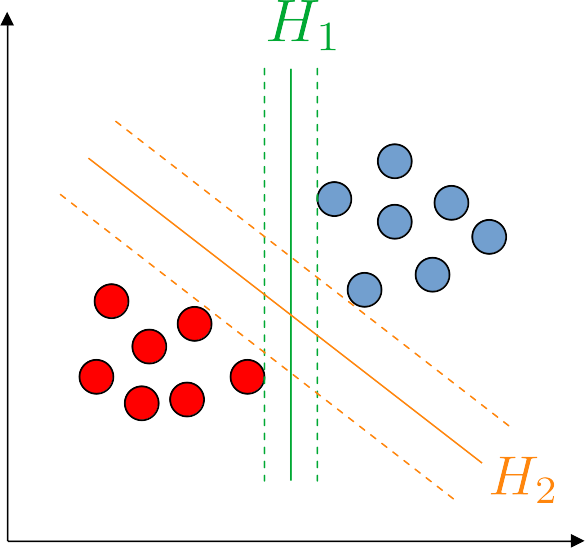
\includegraphics[height=5cm]{./pic/PnmhVqej.png}}
	\caption{資料集中不同的分割線}
	\label{fig:SVMBestSeparte}
\end{figure}

\begin{figure}[H]
	\centerline{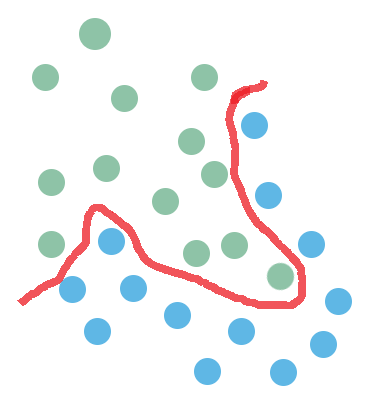
\includegraphics[height=5cm]{pic/unlinear.PNG}}
	\caption{線性不可分示意圖}
	\label{fig:LinearUnseparable}
\end{figure}

\section{演算法參數定義與流程}



\begin{figure}[H]
	\centerline{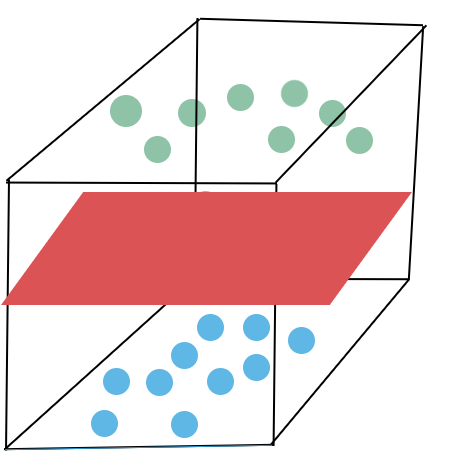
\includegraphics[height=5cm]{pic/over space.PNG}}
	\caption{超空間示意圖}
	\label{fig:Hyperspace}
\end{figure}
\label{sec:background}

\section{核函數(kernel function)}

\begin{enumerate}
	\item
	      Linear Kernel
	      \begin{equation}
		      \label{eqn:LinearKernel}
		      K(x,x')=x^Tx'
	      \end{equation}

\begin{figure}[H]
	\centerline{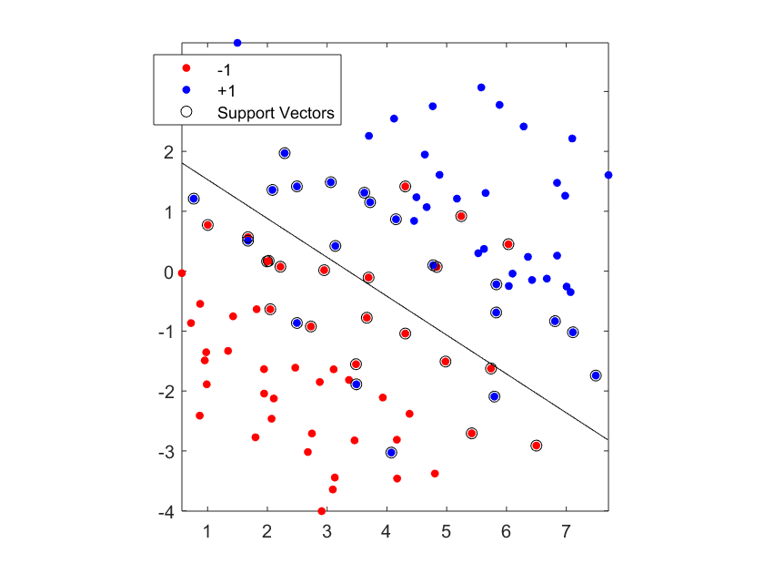
\includegraphics[height=5cm]{pic/linear kernel.png}}
	\caption{linear kernel示意圖}
	\label{fig:linear kernel}
\end{figure}

	\item
	      Radial Basis Function Kernel
	      \begin{table}[h!]
		      \centering
		      \label{tab:rbf_table}
		      \begin{tabular}{ccc}
\toprule
  & RBF的名字 & 方程式 (\(r = ||\mathbf{c-x_i}||\) )   \\ 
\midrule
  & Gaussian Function  & \(h(x)=\phi(r) = e^{-\varepsilon r}\)      \\ \\ 
  & Linear radial Function  & \(h(x)=\phi(r) = r\)      \\ \\
  & Multiquadric   & \(h(x)=\phi(r) = \sqrt{1+(\varepsilon r)^2}\)       \\ \\
  & Inverse quadric  &  \(h(x)=\phi(r) = \frac{1}{1+(\varepsilon r)^2}\)     \\ \\ 
  & Inverse Multiquadric  &  \(h(x)=\phi(r) = \frac{1}{\sqrt{1+(\varepsilon r)^2}}\)     \\
\bottomrule
\end{tabular}

		      \caption{常見的Radial Basis Function}
	      \end{table}
\begin{figure}[H]
	\centerline{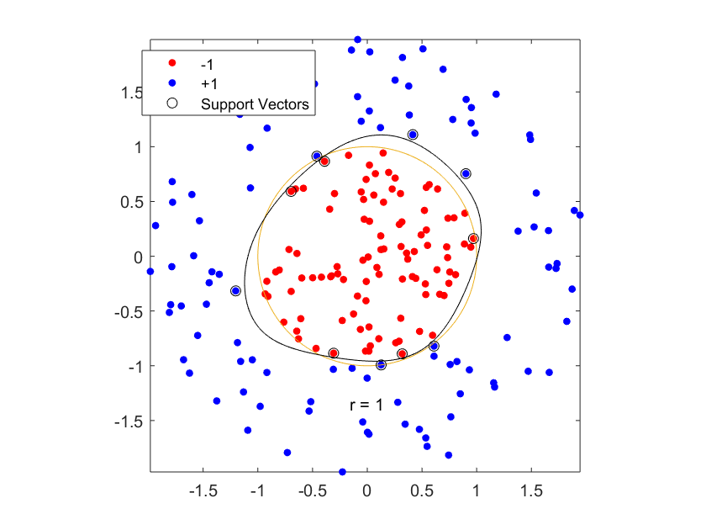
\includegraphics[height=5cm]{pic/Radial Basis Function Kernel.png}}
	\caption{Radial Basis Function Kernel示意圖}
	\label{fig:Radial Basis}
\end{figure}
	\item
	      Sigmoid Kernel
	      \begin{equation}
		      \label{eqn:Sigmoid Kerne}
		      S(t)=\frac{1}{1+e^{-t}}
	      \end{equation}
\begin{figure}[H]
	\centerline{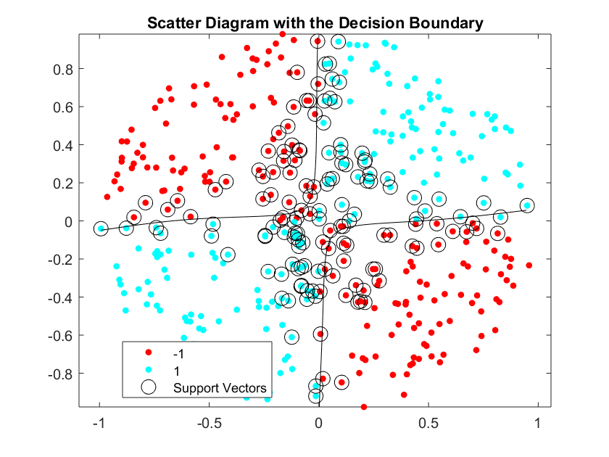
\includegraphics[height=5cm]{pic/Sigmoid Kernel.png}}
	\caption{Sigmoid Kernel示意圖}
	\label{Sigmoid Kernel}
\end{figure}


\end{enumerate}


